\chapter{Reaching II: Real-robot reaching}

After the first experiment, we know that a simulated robot can move its
end-effector to goal positions arbitrarily set within the workspace.  Now, to
investigate whether the same method would generalize to real robotic arms,
robots were set up to perform a reaching task, where a central server
maintained a replay buffer, parameters, and executed training.  Data collection
was distributed over three robots with respective computers.

\section{Method}

\subsection{Definition of the MDP}

The same definition used in the previous experiment was used, with the
exception of a smaller action space for the sake of smoother trajectories:
\begin{equation}
    \mathcal{A} = \lbrace \mathbf{a} \in \mathbb{R}^2 \mid ||\mathbf{a}|| < 0.01 \rbrace
\end{equation}
Also, the dynamics of the system can of course no longer be defined since
it is a real system.

\subsection{Environment}

Instead of a simulated environment, a real robotic system was used. Three 3-DoF
robotic arms controlled by cartesian commands were controlled by policies
running on dedicated computers. The state was observed by reading servo angles
and calculating cartesian coordinates using forward kinematics. The environment
is still 2-dimensional by keeping the $z$-coordinate fixed.

\subsection{Algorithms}

The same NAF implementation as in the previous simulated experiment was used,
but with the modifications for distributed data collection. The action output
$\mu$ of the network was scaled to have maximum norm $0.01$ to enforce smoother
movements. The policy was trained on a separate server equipped with a GPU. For
every arm, there was one dedicated computer each that evaluated the latest
policy given the arm pose and sent the transitions to the server.  The entire
setup (excluding server) is shown in the bottom part of figure
\ref{fig:workspace_lidar_place}. In order to facilitate communication of
recorded state transitions and fetching updated parameters, a server was
implemented enabling PUT and GET requests from the local workers.

Action steps could only be done at approx. $2-4$ Hz, not including arm
re-positioning for environment reset, making re-runs from scratch time
consuming. Therefore, data gathering was first run on the three robots for $4$
hours without policy updates, resulting in approximately $80k$ state
transitions. The actions during the data collection-only phase were randomly
drawn from $\mathcal{N}(\mathbf{0}, 0.005^2 \mathbf{I})$, and when the robot
arm reached outside the workspace, or reached within $1$ cm of the target, the
end-effector was replaced at a new random starting position. The commands were
2-dimensional vectors representing the relative movement in $x$ and $y$
direction respectively. When training of the parameters was started on the
server, the robots kept collecting and pushing data to the server, and
synchronized parameters before each reset of the end-effector position. During
this phase, noise was added to the policy during every 3 out of 4 runs, while
every 1 out 4 runs the policy was evaluated without noise in order to track
progress.

\section{Results}

The performance of the policy was evaluated by measuring the average distance
to the target position on the last state before every reset. The progress of
this metric is shown in figure \ref{fig:uarm_moving_goal_progress}, here shown
with a running mean of width $128$. The trained policy and value function are
shown in figure \ref{fig:uarm_moving_goal_policy}. The distributed version of
NAF solves the task of approaching arbitrarily set goals on a set of
distributed real-world robots.

\begin{figure}[h!]
    \centering
    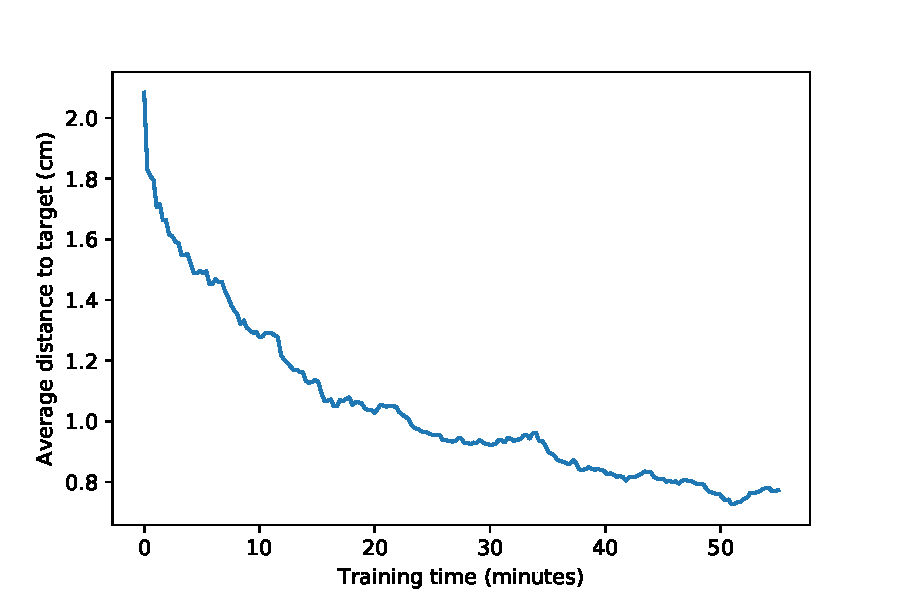
\includegraphics[width=0.50 \textwidth]{res/uarm_moving_goal_progress.pdf}

    \caption{Average final distance of end-effector to randomly set target
    poses learned using a pool of robots collecting experience. NAF was used
    for training the policy on a separate server from a growing set of
    transitions sent from the collecting robots.}
    \label{fig:uarm_moving_goal_progress}
    
\end{figure}

\begin{figure}[h]
    \centering
    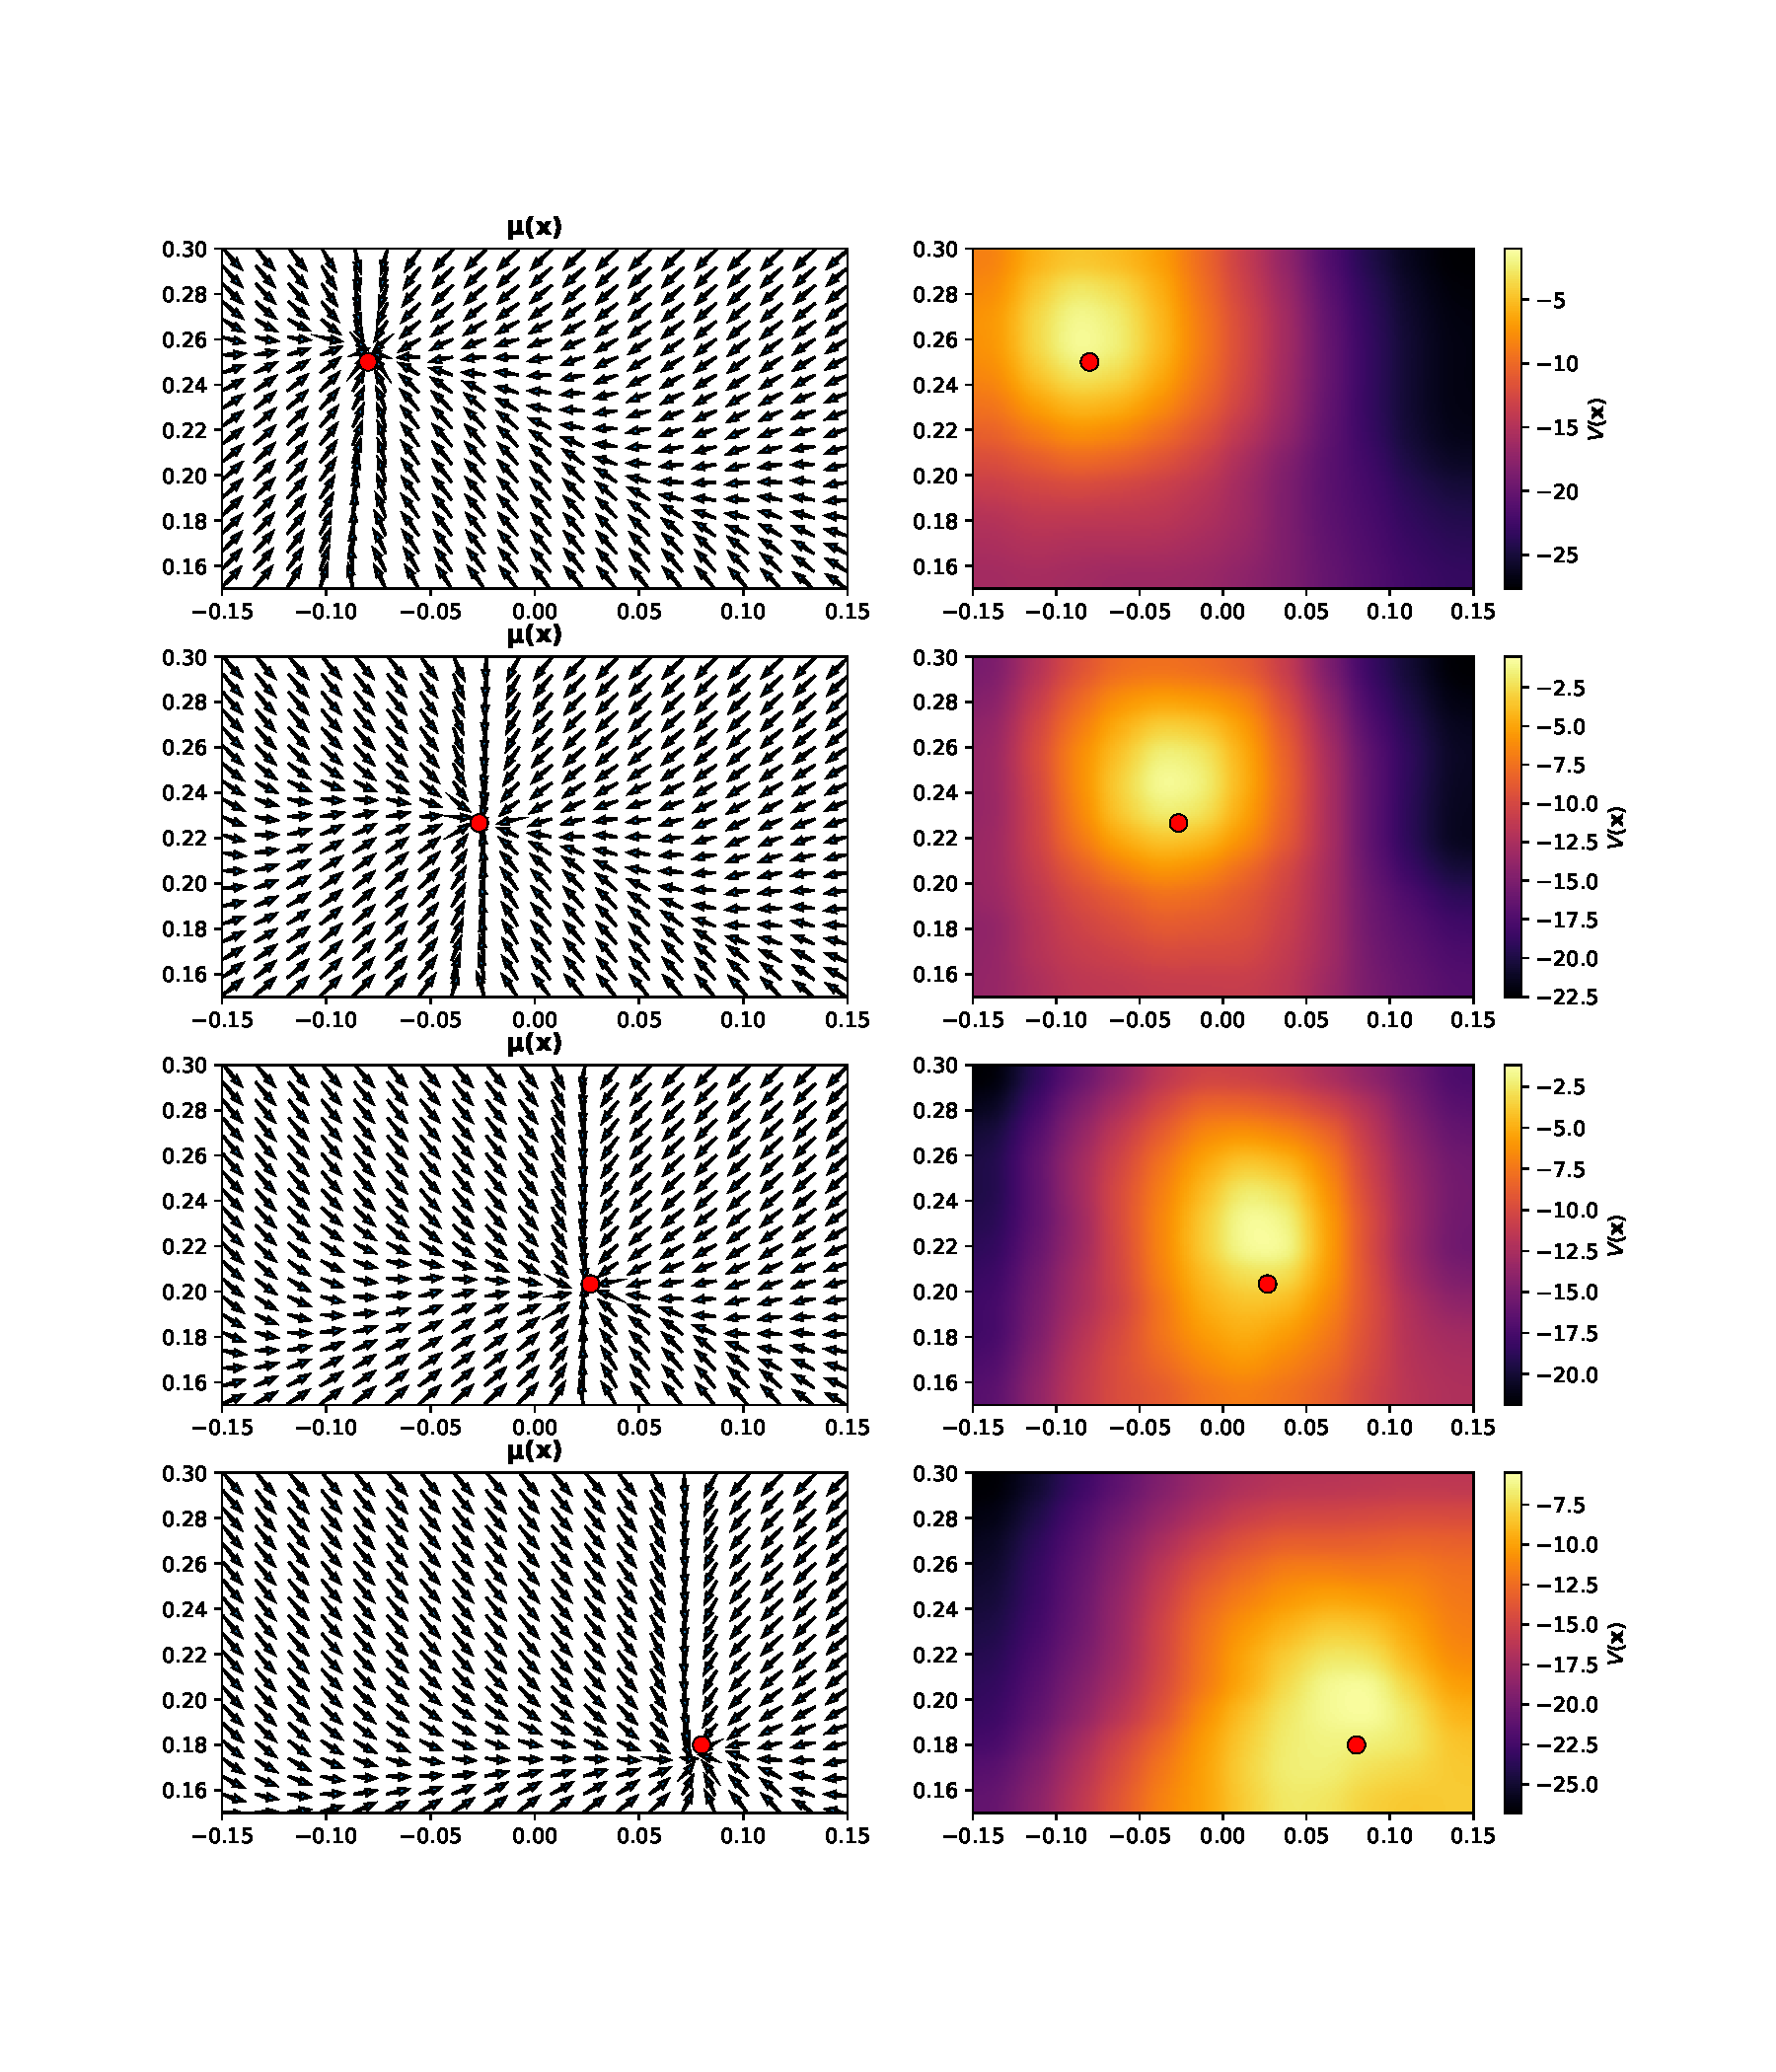
\includegraphics[width=\textwidth]{res/multiple_goals_uarm.pdf}

    \caption{Learned policy using NAF with distributed collection of experience
    from real-world robots.}

    \label{fig:uarm_moving_goal_policy}
    
\end{figure}

%\begin{figure}[h]
%    \centering
%    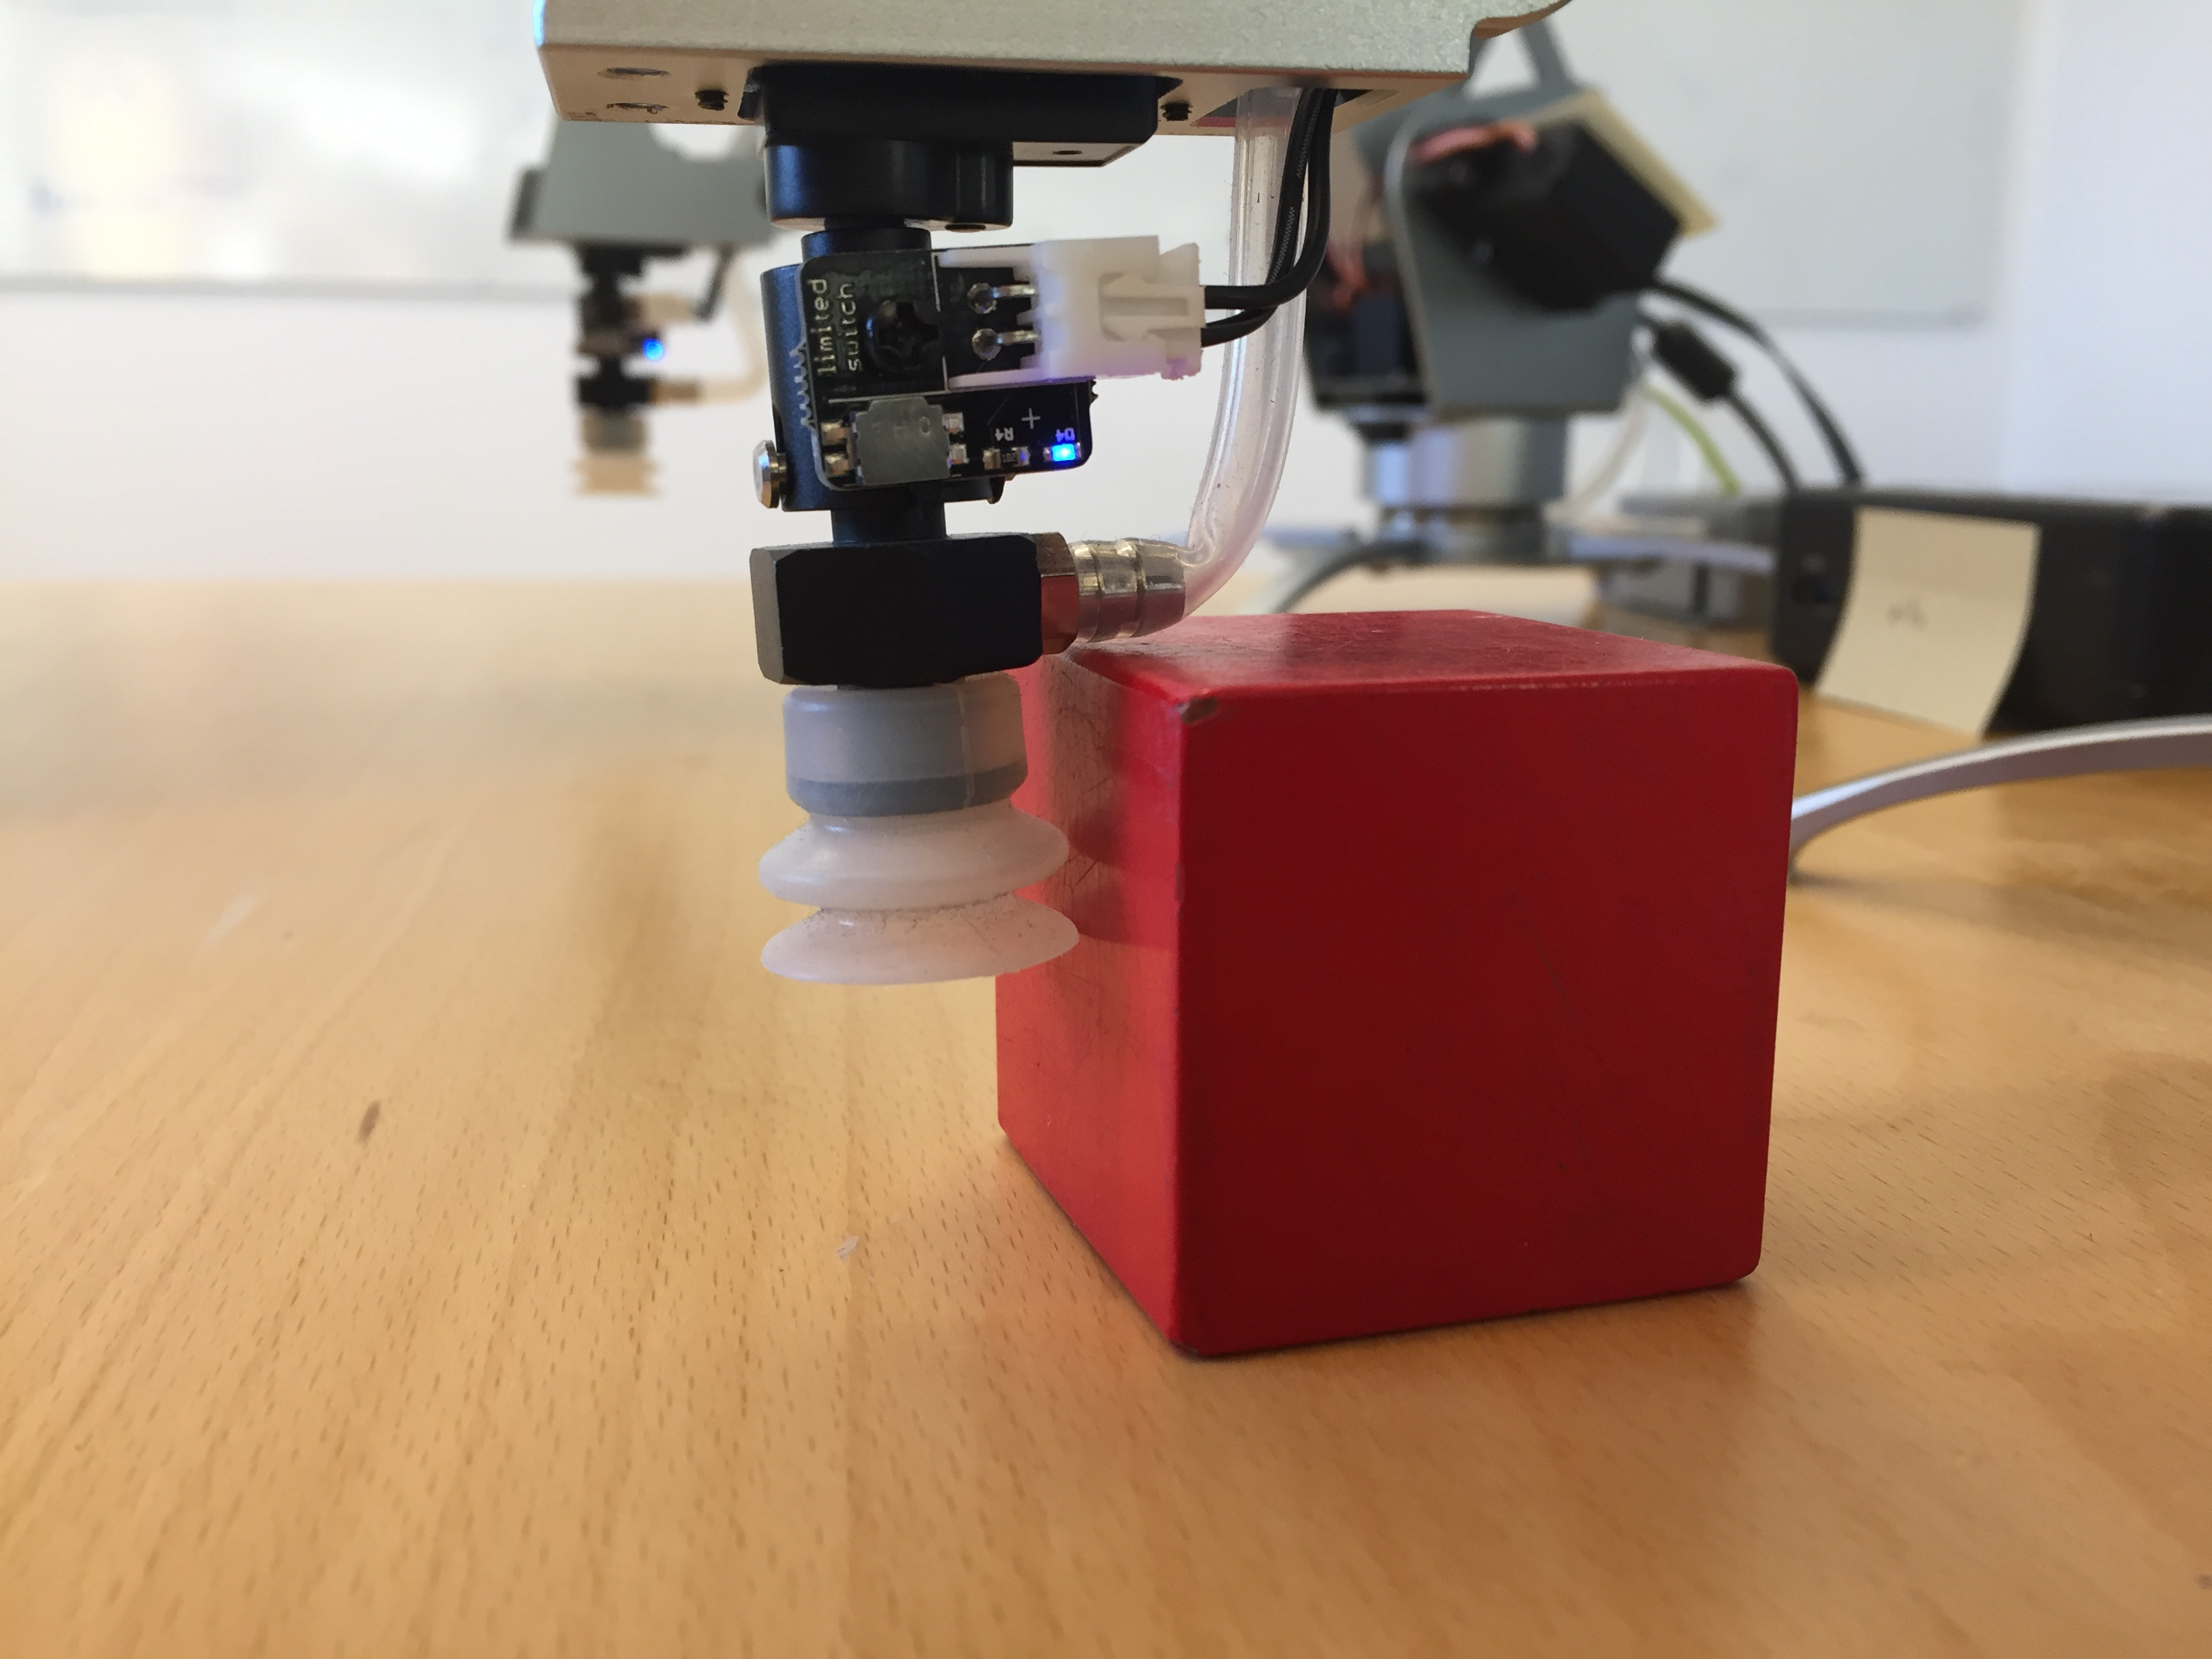
\includegraphics[width=0.40 \textwidth]{res/eef_cube_low.jpg}
%    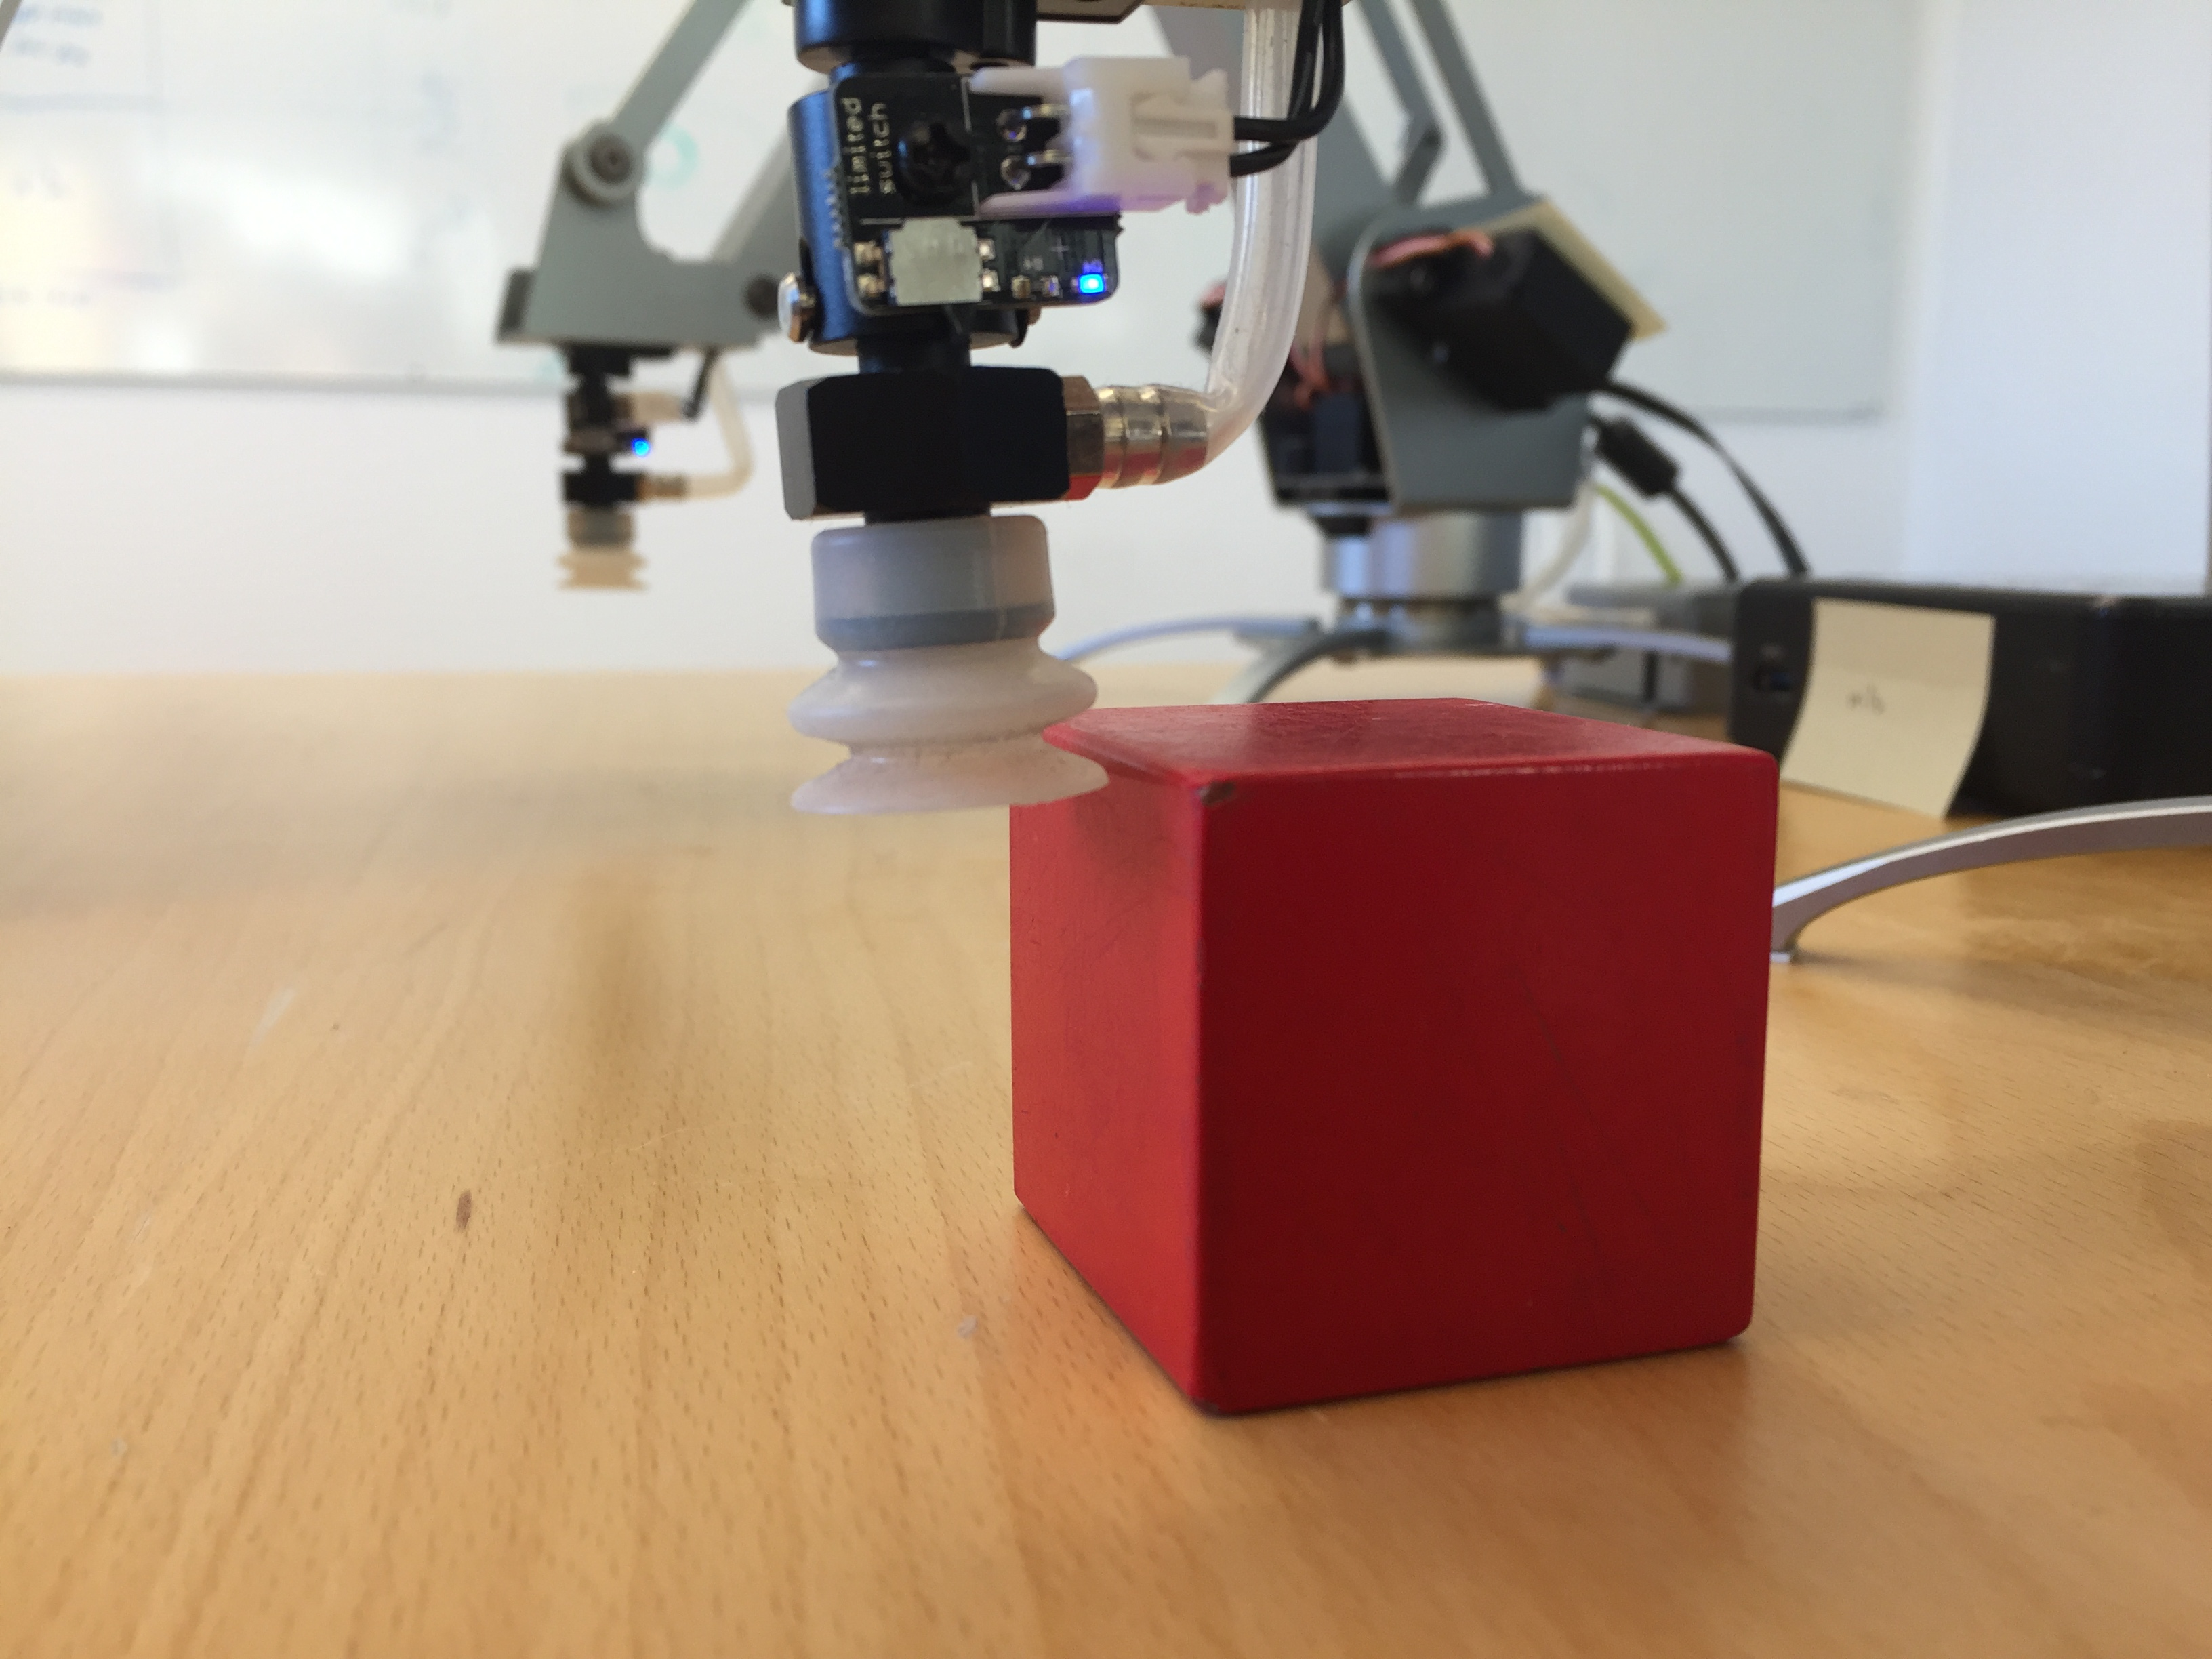
\includegraphics[width=0.40 \textwidth]{res/eef_cube_high.jpg}
%
%    \caption{Possible $z$-values of the eef. TODO: Finish/polish this}
%    
%\end{figure}
